\section{问题三的模型建立与求解}

\subsection{优化模型的建立}

以矩形海域中心为原点建立水平坐标系，$x$ 向东为正（东侧为浅水），$y$ 向北为正。海域东西边界为 $x_{\min}=-3704\text{ m}$、$x_{\max}=3704\text{ m}$，南北边界为 $y_{\min}=-1852\text{ m}$、$y_{\max}=1852\text{ m}$（$1$ 海里 $=1852$ 米）。

由于海底为西深东浅的单一平面，等深线为南北向直线。测线沿等深线南北向布设时，每条线上的水深恒定，问题可降为一维布线。设第 $i$ 条测线坐标为 $x_i$，其两侧水平半覆盖宽度为

\begin{equation}
  B_W(x_i)=\frac{D(x_i)\sin\phi\cos\alpha}{\cos(\phi+\alpha)},\qquad
  B_E(x_i)=\frac{D(x_i)\sin\phi\cos\alpha}{\cos(\phi-\alpha)},
\end{equation}

其中 $D(x_i)=110-x_i\tan\alpha$。相邻条带的代数重叠宽度与重叠率为

\begin{equation}
  O_i=B_E(x_{i-1})+B_W(x_i)-(x_i-x_{i-1}),\qquad
  \eta_i=\frac{O_i}{B_W(x_i)+B_E(x_i)}\times100\%.
\end{equation}

为保证完全覆盖，首条测线西侧覆盖边界应覆盖西边界，末条测线东侧覆盖边界应覆盖东边界：

\begin{equation}
  x_1-B_W(x_1)\le x_{\min},\qquad
  x_n+B_E(x_n)\ge x_{\max}.
\end{equation}

相邻重叠率应满足 $10\%\le\eta_i\le20\%$。每条测线贯穿矩形，长度均为 $y_{\max}-y_{\min}=3704\text{ m}$，故总长度最小等价于测线数最少。问题三转化为

\begin{equation}
  \min n,\qquad \text{s.t.}\quad
  \begin{aligned}[t]
    &10\%\le\eta_i\le20\%,\quad i=2,\dots,n,\\
    &x_1-B_W(x_1)\le x_{\min},\\
    &x_n+B_E(x_n)\ge x_{\max}.
  \end{aligned}
  \label{eq:q3_opt}
\end{equation}

\subsection{贪心递推求解}

为最小化测线数，第一步将首条测线尽可能向东放置，同时令其西侧覆盖边界正好覆盖西边界，即求解 $x_1-B_W(x_1)=x_{\min}$。此后每一步在保证与前一条测线之间无漏测的前提下取最大可行间距，即令重叠率取约束下限 $\eta_i=10\%$，用二分法递推 $x_i$，直至末条测线覆盖东边界。

\subsection{求解结果}

程序得到推荐方案：测线方向为南北向、平行等深线，共 $34$ 条；每条测线长 $2$ 海里，总长度 $68.00$ 海里，即 $125936.00\text{ m}$。布设俯视图见图 4，相邻间距与重叠率校验见图 5。

\begin{figure}[H]
  \centering
  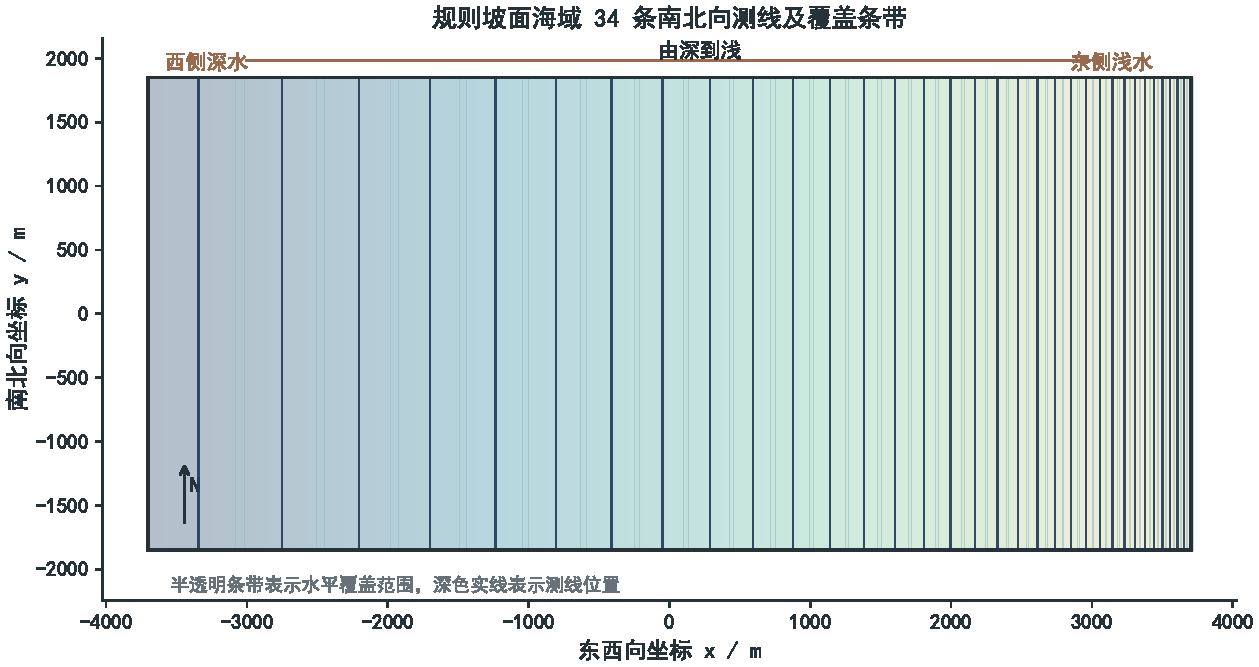
\includegraphics[width=0.9\textwidth]{../figures/q3/fig_q3_layout.pdf}
  \caption{34 条南北向测线在矩形海域内的布设}
  \label{fig:q3_layout}
\end{figure}

\begin{figure}[H]
  \centering
  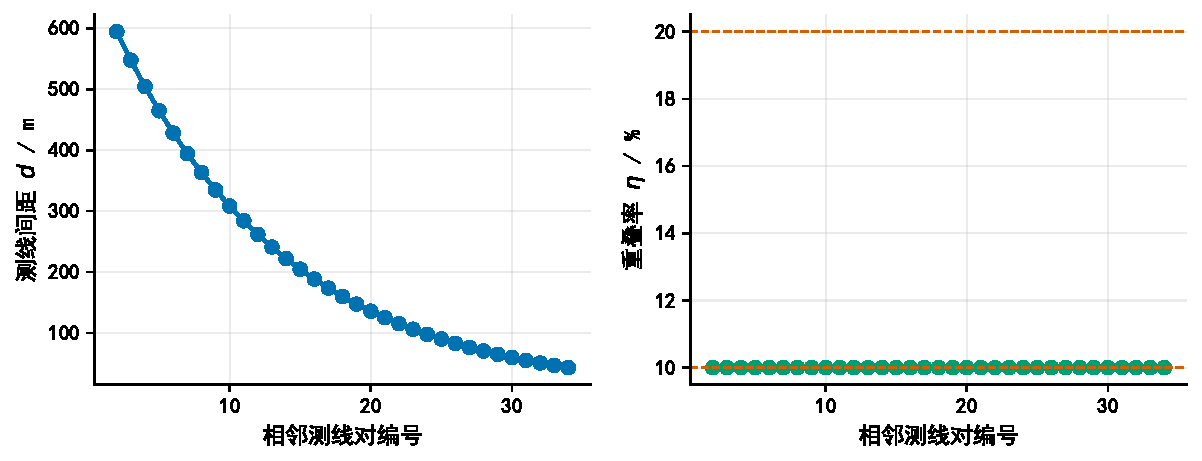
\includegraphics[width=0.95\textwidth]{../figures/q3/fig_q3_spacing.pdf}
  \caption{相邻测线间距与重叠率随测线对编号的变化}
  \label{fig:q3_spacing}
\end{figure}

\subsection{模型验证与本问结论}

完全覆盖检验表明，首条测线西覆盖边界为 $-3704.00\text{ m}$、末条测线东覆盖边界为 $3719.41\text{ m}$，东西方向无漏测；逐对复算 $33$ 个相邻重叠率均为 $10.00\%$，满足 $10\%\sim20\%$。最小条数检验表明，若少一条测线，在同样取最大可行间距的情况下最东覆盖边界仅为 $3678.24\text{ m}$，距东边界仍有 $25.76\text{ m}$ 缺口，因此 $33$ 条不可行。故该方案在所选方向与布线规则下测线数已不可再减少。
